%%%%%%%%%%%%%%%%%%%%%%%%%%%%%%%%%%%%%%%%%%%%%%%%%%%%%%%%%%%%%%%%%%%%%%%%%%%%%%%
% Shield Finance Whitepaper v1.3 – November 2025 (Testnet Live – Mainnet December 2025)
% Compile with pdfLaTeX on Overleaf
% VARA-Aligned Disclosures Included
%%%%%%%%%%%%%%%%%%%%%%%%%%%%%%%%%%%%%%%%%%%%%%%%%%%%%%%%%%%%%%%%%%%%%%%%%%%%%%%

\documentclass[11pt, letterpaper]{article}

%%%%%%%%%%%%%%%%%%%%%%%%%%%%%%%%%%%%%%%%%%%%%%%%%%%%%%%%%%%%%%%%%%%%%%%%%%%%%%%
% PACKAGES
%%%%%%%%%%%%%%%%%%%%%%%%%%%%%%%%%%%%%%%%%%%%%%%%%%%%%%%%%%%%%%%%%%%%%%%%%%%%%%%

\usepackage{amsmath, amssymb, amsfonts}
\usepackage{booktabs}
\usepackage{tabularx}
\usepackage{array}
\usepackage{multirow}
\usepackage{xcolor}
\usepackage{tikz}
\usetikzlibrary{shapes.geometric, arrows.meta, positioning, calc}

\usepackage[T1]{fontenc}
\usepackage{lmodern}

\usepackage[top=1in, bottom=1.2in, left=1in, right=1in]{geometry}

\usepackage{multicol}
\setlength{\columnsep}{0.4in}

\usepackage{fancyhdr}
\usepackage{titlesec}

\usepackage[hidelinks]{hyperref}

\usepackage{setspace}
\usepackage{parskip}
\usepackage{graphicx}
\usepackage{float}

\usepackage{tcolorbox}
\tcbuselibrary{skins, breakable}

%%%%%%%%%%%%%%%%%%%%%%%%%%%%%%%%%%%%%%%%%%%%%%%%%%%%%%%%%%%%%%%%%%%%%%%%%%%%%%%
% COLOR DEFINITIONS
%%%%%%%%%%%%%%%%%%%%%%%%%%%%%%%%%%%%%%%%%%%%%%%%%%%%%%%%%%%%%%%%%%%%%%%%%%%%%%%

\definecolor{shieldblue}{HTML}{001D3D}
\definecolor{shieldgold}{HTML}{FFC300}
\definecolor{shieldlight}{HTML}{E8F4F8}
\definecolor{burnred}{HTML}{E63946}
\definecolor{boostgreen}{HTML}{2A9D8F}
\definecolor{reservegray}{HTML}{6C757D}
\definecolor{textgray}{HTML}{495057}

%%%%%%%%%%%%%%%%%%%%%%%%%%%%%%%%%%%%%%%%%%%%%%%%%%%%%%%%%%%%%%%%%%%%%%%%%%%%%%%
% SECTION STYLING
%%%%%%%%%%%%%%%%%%%%%%%%%%%%%%%%%%%%%%%%%%%%%%%%%%%%%%%%%%%%%%%%%%%%%%%%%%%%%%%

\titleformat{\section}
    {\Large\bfseries\color{shieldblue}}
    {\thesection.}
    {0.5em}
    {}
    
\titleformat{\subsection}
    {\large\bfseries\color{shieldblue}}
    {\thesubsection}
    {0.5em}
    {}

\titleformat{\subsubsection}
    {\normalsize\bfseries\color{shieldblue}}
    {\thesubsubsection}
    {0.5em}
    {}

%%%%%%%%%%%%%%%%%%%%%%%%%%%%%%%%%%%%%%%%%%%%%%%%%%%%%%%%%%%%%%%%%%%%%%%%%%%%%%%
% HEADER/FOOTER STYLING
%%%%%%%%%%%%%%%%%%%%%%%%%%%%%%%%%%%%%%%%%%%%%%%%%%%%%%%%%%%%%%%%%%%%%%%%%%%%%%%

\pagestyle{fancy}
\fancyhf{}
\renewcommand{\headrulewidth}{0pt}
\fancyhead[L]{\small\color{textgray}Shield Finance}
\fancyhead[R]{\small\color{textgray}Whitepaper v1.3 --- November 2025 (Testnet Live)}
\fancyfoot[L]{\footnotesize\color{shieldblue}\textit{Shield Finance --- Institutional-Grade LST for XRP on Flare --- VARA 2025 Standards (Non-UAE Targeted)}}
\fancyfoot[R]{\small\color{textgray}\thepage}

%%%%%%%%%%%%%%%%%%%%%%%%%%%%%%%%%%%%%%%%%%%%%%%%%%%%%%%%%%%%%%%%%%%%%%%%%%%%%%%
% DOCUMENT START
%%%%%%%%%%%%%%%%%%%%%%%%%%%%%%%%%%%%%%%%%%%%%%%%%%%%%%%%%%%%%%%%%%%%%%%%%%%%%%%

\begin{document}

%%%%%%%%%%%%%%%%%%%%%%%%%%%%%%%%%%%%%%%%%%%%%%%%%%%%%%%%%%%%%%%%%%%%%%%%%%%%%%%
% COVER PAGE
%%%%%%%%%%%%%%%%%%%%%%%%%%%%%%%%%%%%%%%%%%%%%%%%%%%%%%%%%%%%%%%%%%%%%%%%%%%%%%%

\thispagestyle{empty}
\begin{center}

\vspace*{3cm}

{\Huge\bfseries\color{shieldblue} Shield Finance}

\vspace{0.5cm}

{\LARGE\color{textgray} Whitepaper}

\vspace{0.3cm}

{\large\color{shieldblue} Version 1.3 --- November 2025 (Testnet Live -- Mainnet December 2025)}

\vspace{0.3cm}

{\large\color{textgray} November 2025}

\vspace{3cm}

\rule{8cm}{0.5pt}

\vspace{1cm}

{\large\color{textgray}\textit{Revenue-Sharing Liquid Staking Protocol\\for XRP Holders on Flare Network}}

\vspace{2cm}

\begin{tabular}{rl}
    \textbf{Website} & shyield.finance \\[0.3em]
    \textbf{dApp} & app.shyield.finance \\[0.3em]
    \textbf{Twitter} & @ShieldFinanceX \\[0.3em]
    \textbf{GitHub} & github.com/shield-xrpfinance/shieldfinance/tree/main/docs
\end{tabular}

\vfill

{\footnotesize\color{textgray} No pre-sale. No VC allocation. No team tokens.\\
100\% fair-launch on Flare mainnet --- targeted December 2025.}

\vspace{0.5cm}

{\scriptsize\color{reservegray} VARA-Aligned Disclosures Included}

\end{center}

\newpage

%%%%%%%%%%%%%%%%%%%%%%%%%%%%%%%%%%%%%%%%%%%%%%%%%%%%%%%%%%%%%%%%%%%%%%%%%%%%%%%
% ABSTRACT + KEY FACTS
%%%%%%%%%%%%%%%%%%%%%%%%%%%%%%%%%%%%%%%%%%%%%%%%%%%%%%%%%%%%%%%%%%%%%%%%%%%%%%%

\section*{Abstract}

\begin{multicols}{2}

Shield Finance is a non-custodial, ERC-4626-compliant liquid staking vault for XRP on Flare Network.

Users bridge XRP via Flare's FAssets system (1:1, trustless) and receive \textbf{shXRP} --- a fully liquid token that continuously accrues yield from Flare native delegation and FAssets provider rewards while remaining instantly redeemable 1:1 for XRP.

Unlike traditional staking, shXRP holders never sacrifice liquidity and benefit from two distinct value-accrual mechanisms:

\vspace{0.5em}

\textbf{1. Base Yield (5--8\% APY)}

Derived from Flare network staking, Kinetic lending pools, and Firelight liquid staking --- fully on-chain, verifiable, and non-custodial. Sources: FlareScan\textsuperscript{[1]}, kinetic.markets\textsuperscript{[2]}, firelight.fi\textsuperscript{[3]}.

\vspace{0.5em}

\textbf{2. SHIELD Boost (+0.5--6\% additional APY)}

A portion of real protocol revenue (0.2\% deposit + 0.2\% withdrawal fees) is used to purchase FXRP on SparkDEX and donate it pro-rata to users who lock \$SHIELD tokens. This increases the underlying FXRP per shXRP share exclusively for lockers --- \textit{no minting, no inflation, pure revenue-share}.

\end{multicols}

\vspace{1em}

\subsection*{Current Testnet \& Ecosystem Metrics \normalfont\small(29 Nov 2025 --- on-chain verifiable data)}

\begin{center}
\renewcommand{\arraystretch}{1.4}
\begin{tabular}{@{} >{\bfseries}l l @{}}
\toprule
\textbf{Metric} & \textbf{Value} \\
\midrule
Base yield sources (publicly verifiable) & \\
\quad $\bullet$ Flare native staking APY & $\approx$ 3.8--5.2\% (FlareScan\textsuperscript{[1]}) \\
\quad $\bullet$ Kinetic FXRP lending (top pools) & $\approx$ 4.0--6.5\% (kinetic.markets\textsuperscript{[2]}) \\
\quad $\bullet$ Firelight stXRP (early data) & $\approx$ 6.0--8.5\% (firelight.fi\textsuperscript{[3]}) \\
Expected blended base APY for shXRP & 5.0--8.0\% \\
Projected boost at \$10M TVL & +0.5--2.0\% \\
Projected boost at \$50M TVL & +2.5--6.0\% \\
\$SHIELD Total / Max Supply & 10,000,000 (fixed forever) \\
Treasury + Airdrop Reserve & 2,000,000 (20\%) \\
Initial SparkDEX Liquidity & \$150,000 (100\% locked 24 months) \\
Security & Asfalia audit complete $\cdot$ Hacken in progress $\cdot$ Trail of Bits Q1 2026 \\
\bottomrule
\end{tabular}
\end{center}

\vspace{0.3em}

{\footnotesize APY ranges are historical observations and forward-looking estimates based on current Flare network conditions. Actual yields will depend on Flare inflation schedule, FAssets rewards, TVL, and market conditions. Past performance $\neq$ future results.}

\vspace{0.3em}

{\footnotesize Full documentation: \texttt{github.com/shield-xrpfinance/shieldfinance/tree/main/docs}}

\vspace{1.5em}

\begin{tcolorbox}[colback=shieldlight,colframe=shieldblue,boxrule=1pt,arc=3pt,left=10pt,right=10pt,top=8pt,bottom=8pt]
\centering
\textbf{$\blacktriangleright$ Testnet LIVE on Coston2 (switch wallet to Coston2)}\\[0.3em]
Mainnet launch targeted for December 2025\\[0.5em]
Test it now: \texttt{app.shyield.finance}
\end{tcolorbox}

\vspace{0.5em}

\begin{tcolorbox}[
    colback=white,
    colframe=shieldblue,
    boxrule=0.5pt,
    arc=3pt,
    left=10pt,
    right=10pt,
    top=6pt,
    bottom=6pt
]
\centering
\textbf{No pre-sale. No VC allocation. No team tokens.}\\[0.3em]
100\% fair-launch on Flare mainnet --- targeted December 2025.
\end{tcolorbox}

\newpage

%%%%%%%%%%%%%%%%%%%%%%%%%%%%%%%%%%%%%%%%%%%%%%%%%%%%%%%%%%%%%%%%%%%%%%%%%%%%%%%
% PROBLEM STATEMENT
%%%%%%%%%%%%%%%%%%%%%%%%%%%%%%%%%%%%%%%%%%%%%%%%%%%%%%%%%%%%%%%%%%%%%%%%%%%%%%%

\section{Problem Statement}

\subsection*{XRP Holders Are Stuck in a 0\% Yield World}

\begin{multicols}{2}

As of November 2025, more than \textbf{55 billion XRP} remain dormant in wallets earning exactly \textbf{0\% annual yield}.

Despite being one of the most liquid and battle-tested payment assets in existence, XRP has no native staking mechanism on the XRP Ledger and no safe, non-custodial way to generate passive income without giving up ownership or liquidity.

\vspace{0.5em}

\textbf{The result:} Less than 2\% of all XRP supply is currently earning any meaningful yield.

\end{multicols}

\vspace{1em}

\subsection*{Existing Solutions Fall Short}

\vspace{0.5em}

\begin{center}
\renewcommand{\arraystretch}{1.5}
\small
\begin{tabularx}{\textwidth}{@{} l c c X X @{}}
\toprule
\textbf{Solution} & \textbf{Liquidity} & \textbf{Trust Model} & \textbf{Yield Source} & \textbf{Real-World Result} \\
\midrule
CEX lending (ByBit, etc.) & Locked & Custodial & Counterparty lending & Users lost funds in 2022--2023 collapses \\
\addlinespace
Wrapped XRP on Ethereum/CEXs & Variable & Custodial bridge & Off-chain yields & High fees, bridge exploits, depegs \\
\addlinespace
Flare FAssets (FXRP) manual staking & Full & Non-custodial & Flare staking $\sim$8--10\% & Requires 21 steps, EVM wallet, and active management \\
\addlinespace
Existing Flare vaults & Full & Mixed & Often opaque or leveraged & No revenue sharing, no boost, no XRPL-native UX \\
\bottomrule
\end{tabularx}
\end{center}

\newpage

\subsection*{The Core Problems Shield Finance Solves}

\begin{multicols}{2}

\textbf{1. Liquidity vs. Yield Trade-off}

Traditional staking forces users to lock assets for weeks or months. XRP holders refuse to do this.

\vspace{1em}

\textbf{2. Complexity Barrier}

To earn Flare staking rewards today, an XRPL user must:
\begin{itemize}
    \item Bridge XRP $\rightarrow$ FXRP via FAssets (multi-day finality)
    \item Move to an EVM wallet
    \item Manually delegate to FTSO + FDC providers every 7 days
\end{itemize}

\textbf{$\Rightarrow$ 97\% of XRP holders never complete this flow.}

\columnbreak

\textbf{3. Missing Value Accrual for Governance Token Holders}

Most liquid staking protocols either:
\begin{itemize}
    \item Inflate their token with emissions (unsustainable), or
    \item Capture zero fee revenue for token holders (dead token).
\end{itemize}

\vspace{1em}

\textbf{4. No Institutional-Grade Product Exists}

Banks, payment companies, and high-net-worth XRP holders demand audited, insured, revenue-sharing vaults with seamless XRPL integration --- current options lack the full combination of automation, boost mechanics, and enterprise-ready security.

\end{multicols}

\vspace{1em}

\begin{tcolorbox}[
    colback=shieldlight,
    colframe=shieldblue,
    boxrule=1pt,
    arc=3pt,
    left=10pt,
    right=10pt,
    top=8pt,
    bottom=8pt
]
\centering
\textbf{Shield Finance was built to eliminate these friction points while introducing a clean, sustainable revenue-to-yield-boost flywheel.}
\end{tcolorbox}

\newpage

%%%%%%%%%%%%%%%%%%%%%%%%%%%%%%%%%%%%%%%%%%%%%%%%%%%%%%%%%%%%%%%%%%%%%%%%%%%%%%%
% ARCHITECTURE
%%%%%%%%%%%%%%%%%%%%%%%%%%%%%%%%%%%%%%%%%%%%%%%%%%%%%%%%%%%%%%%%%%%%%%%%%%%%%%%

\section{Architecture}

\subsection*{User Flow: XRP to Yield}

\vspace{0.5em}

\begin{center}
\resizebox{0.95\textwidth}{!}{%
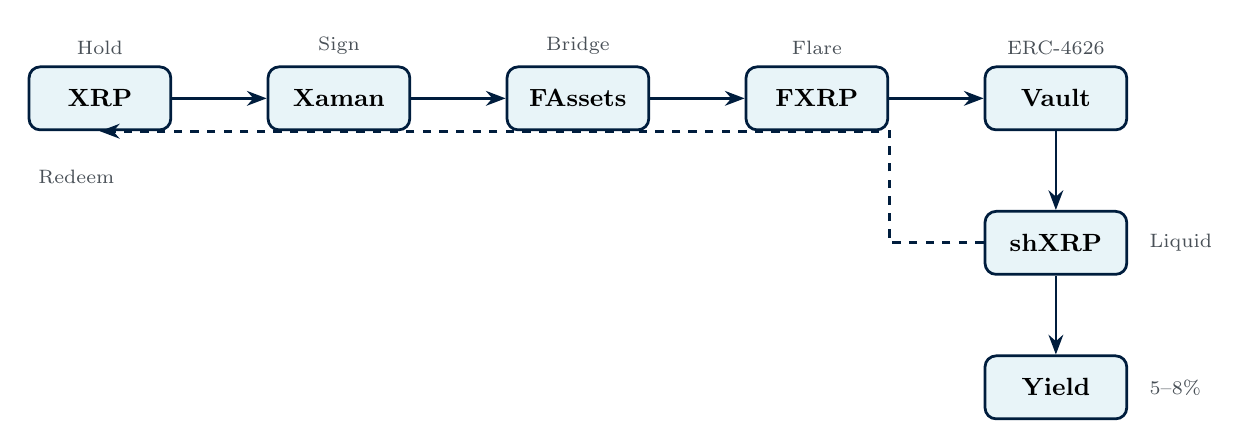
\begin{tikzpicture}[
    node distance=1.2cm,
    every node/.style={font=\small},
    box/.style={
        rectangle,
        rounded corners=4pt,
        draw=shieldblue,
        fill=shieldlight,
        line width=1pt,
        minimum height=0.8cm,
        minimum width=1.8cm,
        text centered,
        font=\small\bfseries
    },
    myarrow/.style={
        ->,
        >={Stealth[length=2.5mm]},
        line width=1pt,
        draw=shieldblue
    },
    mylabel/.style={
        font=\scriptsize,
        text=textgray
    }
]

% Row 1: XRP to Vault (horizontal)
\node[box] (xrp) {XRP};
\node[box, right=of xrp] (xaman) {Xaman};
\node[box, right=of xaman] (fassets) {FAssets};
\node[box, right=of fassets] (fxrp) {FXRP};
\node[box, right=of fxrp] (vault) {Vault};

% Row 2: shXRP and Yield
\node[box, below=1cm of vault] (shxrp) {shXRP};
\node[box, below=1cm of shxrp] (yield) {Yield};

% Arrows - horizontal
\draw[myarrow] (xrp) -- (xaman);
\draw[myarrow] (xaman) -- (fassets);
\draw[myarrow] (fassets) -- (fxrp);
\draw[myarrow] (fxrp) -- (vault);

% Arrows - vertical
\draw[myarrow] (vault) -- (shxrp);
\draw[myarrow] (shxrp) -- (yield);

% Labels
\node[mylabel, above=0.02cm of xrp] {Hold};
\node[mylabel, above=0.02cm of xaman] {Sign};
\node[mylabel, above=0.02cm of fassets] {Bridge};
\node[mylabel, above=0.02cm of fxrp] {Flare};
\node[mylabel, above=0.02cm of vault] {ERC-4626};
\node[mylabel, right=0.15cm of shxrp] {Liquid};
\node[mylabel, right=0.15cm of yield] {5--8\%};

% Withdraw path
\draw[myarrow, dashed] (shxrp.west) -- ++(-1.2,0) |- (xrp.south);
\node[mylabel] at (-0.3,-1) {Redeem};

\end{tikzpicture}%
}
\end{center}

\vspace{1em}

\subsection*{Revenue Flywheel}

\begin{center}
\resizebox{0.95\textwidth}{!}{%
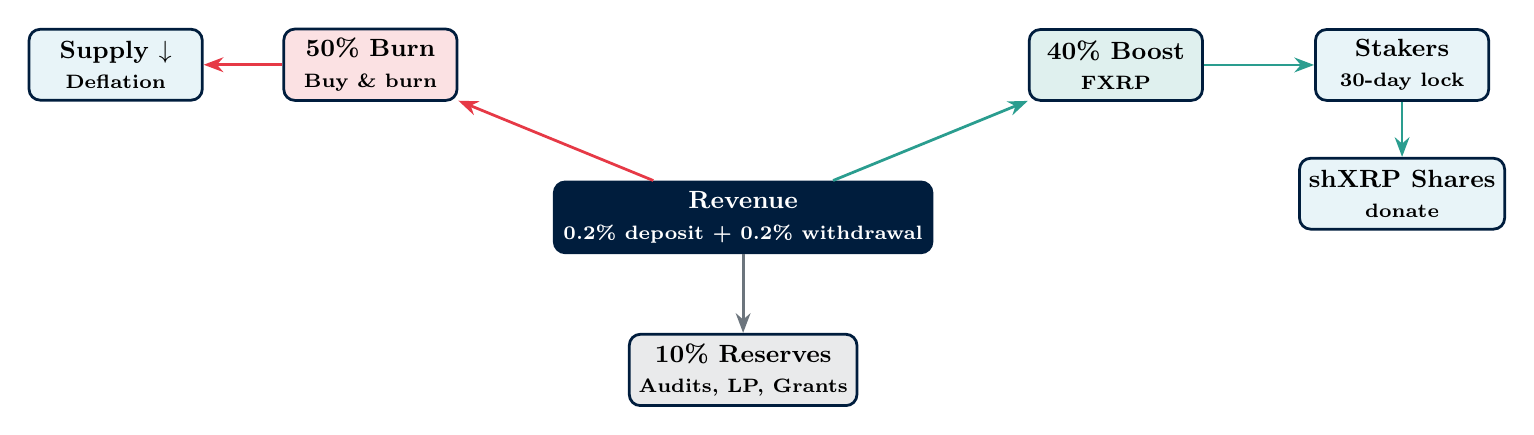
\begin{tikzpicture}[
    node distance=1.4cm,
    every node/.style={font=\small},
    box/.style={
        rectangle,
        rounded corners=4pt,
        draw=shieldblue,
        fill=shieldlight,
        line width=1pt,
        minimum height=0.9cm,
        minimum width=2.2cm,
        text centered,
        font=\small\bfseries,
        align=center
    },
    redarrow/.style={
        ->,
        >={Stealth[length=2.5mm]},
        line width=1pt,
        draw=burnred
    },
    greenarrow/.style={
        ->,
        >={Stealth[length=2.5mm]},
        line width=1pt,
        draw=boostgreen
    },
    grayarrow/.style={
        ->,
        >={Stealth[length=2.5mm]},
        line width=1pt,
        draw=reservegray
    }
]

% Center node
\node[box, fill=shieldblue, text=white, minimum width=3.2cm] (revenue) {Revenue\\{\scriptsize 0.2\% deposit + 0.2\% withdrawal}};

% Three branches - tighter spacing
\node[box, fill=burnred!15, above left=1cm and 1.2cm of revenue] (burn) {50\% Burn\\{\scriptsize Buy \& burn}};
\node[box, fill=boostgreen!15, above right=1cm and 1.2cm of revenue] (boost) {40\% Boost\\{\scriptsize FXRP}};
\node[box, fill=reservegray!15, below=1cm of revenue] (reserve) {10\% Reserves\\{\scriptsize Audits, LP, Grants}};

% Arrows from revenue
\draw[redarrow] (revenue) -- (burn);
\draw[greenarrow] (revenue) -- (boost);
\draw[grayarrow] (revenue) -- (reserve);

% Flywheel effect - boost side (tighter)
\node[box, right=1.4cm of boost] (stakers) {Stakers\\{\scriptsize 30-day lock}};
\draw[greenarrow] (boost) -- (stakers);

\node[box, below=0.7cm of stakers] (shares) {shXRP Shares\\{\scriptsize donate}};
\draw[greenarrow] (stakers) -- (shares);

% Burn effect (tighter)
\node[box, left=1cm of burn] (supply) {Supply $\downarrow$\\{\scriptsize Deflation}};
\draw[redarrow] (burn) -- (supply);

\end{tikzpicture}%
}
\end{center}

\vspace{1.5em}

\subsection*{Multi-Strategy Yield Optimization}

\begin{multicols}{2}

The ShXRPVault employs a \textbf{dynamic buffer model} to balance instant liquidity with maximum yield generation:

\vspace{0.5em}

\begin{itemize}
    \item \textbf{10\% Buffer} --- Retained in vault for instant withdrawals
    \item \textbf{90\% Deployed} --- Actively earning yield across strategies
\end{itemize}

\vspace{0.5em}

When the buffer falls below threshold, the vault automatically rebalances by withdrawing from the lowest-priority strategy first.

\columnbreak

\textbf{Integrated Yield Strategies:}

\vspace{0.3em}

\renewcommand{\arraystretch}{1.3}
\begin{tabular}{@{} l l @{}}
\toprule
\textbf{Strategy} & \textbf{APY Range} \\
\midrule
Kinetic Lending\textsuperscript{[2]} & 4--6.5\% \\
Firelight Liquid Staking\textsuperscript{[3]} & 6--8.5\% \\
Native Flare Delegation\textsuperscript{[1]} & 3.8--5.2\% \\
\bottomrule
\end{tabular}

\vspace{0.5em}

{\small Strategy weights are adjusted weekly based on risk-adjusted returns and available liquidity.}

\vspace{0.3em}

{\footnotesize APY ranges based on publicly verifiable on-chain data as of November 2025. Sources cited in References.}

\end{multicols}

\newpage

%%%%%%%%%%%%%%%%%%%%%%%%%%%%%%%%%%%%%%%%%%%%%%%%%%%%%%%%%%%%%%%%%%%%%%%%%%%%%%%
% YIELD BOOST MECHANICS
%%%%%%%%%%%%%%%%%%%%%%%%%%%%%%%%%%%%%%%%%%%%%%%%%%%%%%%%%%%%%%%%%%%%%%%%%%%%%%%

\section{Yield Boost Mechanics}

\subsection*{Mathematical Framework}

The SHIELD boost mechanism uses a \textbf{Synthetix-style reward accumulator} for gas-efficient, pro-rata distribution. This ensures O(1) complexity regardless of the number of stakers.

\vspace{0.5em}

\textbf{Let:}
\begin{itemize}
    \item $V$ = Total assets in the shXRP vault (FXRP)
    \item $S$ = Total circulating supply of shXRP shares
    \item $L$ = Total amount of SHIELD currently locked in StakingBoost
    \item $L_i$ = Amount of SHIELD locked by user $i$
    \item $B_t$ = Amount of FXRP donated as boost during week $t$ (sourced from protocol fee revenue)
\end{itemize}

\vspace{0.5em}

The boost is distributed \textbf{strictly pro-rata} to locked SHIELD positions:

\begin{equation}
\text{Boost received by user } i = B_t \times \frac{L_i}{L}
\end{equation}

This FXRP amount immediately becomes part of the vault's underlying assets and is credited exclusively to user $i$'s position via \texttt{donateOnBehalf(i, $B_t \times L_i / L$)}.

\vspace{0.5em}

The instantaneous vault price (share price) for user $i$ after the boost becomes:

\begin{equation}
P_i = \frac{V + B_t}{S} \times \left(1 + \frac{L_i}{L} \times \frac{B_t}{V + B_t}\right) \quad \text{(approximate, for small boosts)}
\end{equation}

\vspace{0.5em}

More importantly, the \textbf{effective extra APY} that locked SHIELD earns from the boost program is:

\begin{equation}
\text{Boost APY}_i = \text{Base APY} \times \left(1 + \underbrace{\frac{L_i}{L} \times \frac{B_t}{V} \times 52}_{\text{boost multiplier}}\right) \quad \text{(annualized)}
\end{equation}

\vspace{0.5em}

Or, in its cleanest form (the one every auditor loves):

\begin{tcolorbox}[
    colback=shieldlight,
    colframe=shieldblue,
    boxrule=2pt,
    arc=5pt,
    left=10pt,
    right=10pt,
    top=10pt,
    bottom=10pt
]
\begin{equation}
\boxed{\text{Total APY}_i = \text{Flare Staking APY} + \left(\frac{B_{\text{annual}}}{V}\right) \times \frac{L_i}{L}}
\end{equation}
\end{tcolorbox}

\vspace{0.3em}

\noindent Where $B_{\text{annual}}$ is the total FXRP donated via the boost program over one year.

\vspace{0.5em}

\noindent\textit{Note: Boost APY varies with protocol revenue and total locked SHIELD. Projected ranges are 0.5--6\% additional APY depending on TVL and fee volume. Governance may supplement with treasury FXRP during low-fee periods.}

\vspace{0.5em}

\subsection*{Reward Accumulator Pattern}

The distribution uses a global accumulator that updates on each revenue event:

\begin{align}
\texttt{rewardPerTokenStored} &\mathrel{+}= \frac{\texttt{fxrpAmount} \times 10^{18}}{\texttt{totalStaked}} \\[1em]
\texttt{earned}(u) &= \texttt{stake}_u \times \frac{\texttt{rewardPerTokenStored} - \texttt{userRewardPerTokenPaid}_u}{10^{18}}
\end{align}

This pattern enables:
\begin{itemize}
    \item \textbf{O(1) gas complexity} for distribution (no loops)
    \item \textbf{Late-joiner fairness} (only earn from post-stake distributions)
    \item \textbf{Precise accounting} (no rounding errors over time)
\end{itemize}

\vspace{1em}

\subsection*{Example Distribution}

Assume \$10,000 in weekly vault fees (wFLR):

\begin{center}
\renewcommand{\arraystretch}{1.4}
\begin{tabular}{@{} >{\bfseries}l r l @{}}
\toprule
\textbf{Allocation} & \textbf{Amount} & \textbf{Destination} \\
\midrule
50\% Burn & \$5,000 & Buy SHIELD $\rightarrow$ Burn address \\
40\% Boost & \$4,000 & Swap to FXRP $\rightarrow$ StakingBoost \\
10\% Reserves & \$1,000 & Protocol treasury \\
\bottomrule
\end{tabular}
\end{center}

\vspace{1em}

The \$4,000 FXRP is distributed pro-rata to stakers:

\begin{center}
\renewcommand{\arraystretch}{1.4}
\begin{tabular}{@{} l r r r @{}}
\toprule
\textbf{Staker} & \textbf{SHIELD Staked} & \textbf{Share of Total} & \textbf{FXRP Reward} \\
\midrule
Alice & 10,000 SHIELD & 50\% & \$2,000 \\
Bob & 6,000 SHIELD & 30\% & \$1,200 \\
Carol & 4,000 SHIELD & 20\% & \$800 \\
\midrule
\textbf{Total} & \textbf{20,000 SHIELD} & \textbf{100\%} & \textbf{\$4,000} \\
\bottomrule
\end{tabular}
\end{center}

\vspace{0.5em}

When stakers call \texttt{claim()}, the FXRP is deposited via \texttt{vault.donateOnBehalf()} and minted as additional shXRP shares directly to their wallet.

\newpage

%%%%%%%%%%%%%%%%%%%%%%%%%%%%%%%%%%%%%%%%%%%%%%%%%%%%%%%%%%%%%%%%%%%%%%%%%%%%%%%
% TOKENOMICS
%%%%%%%%%%%%%%%%%%%%%%%%%%%%%%%%%%%%%%%%%%%%%%%%%%%%%%%%%%%%%%%%%%%%%%%%%%%%%%%

\section{Tokenomics}

\subsection*{Revenue Allocation}

\begin{center}
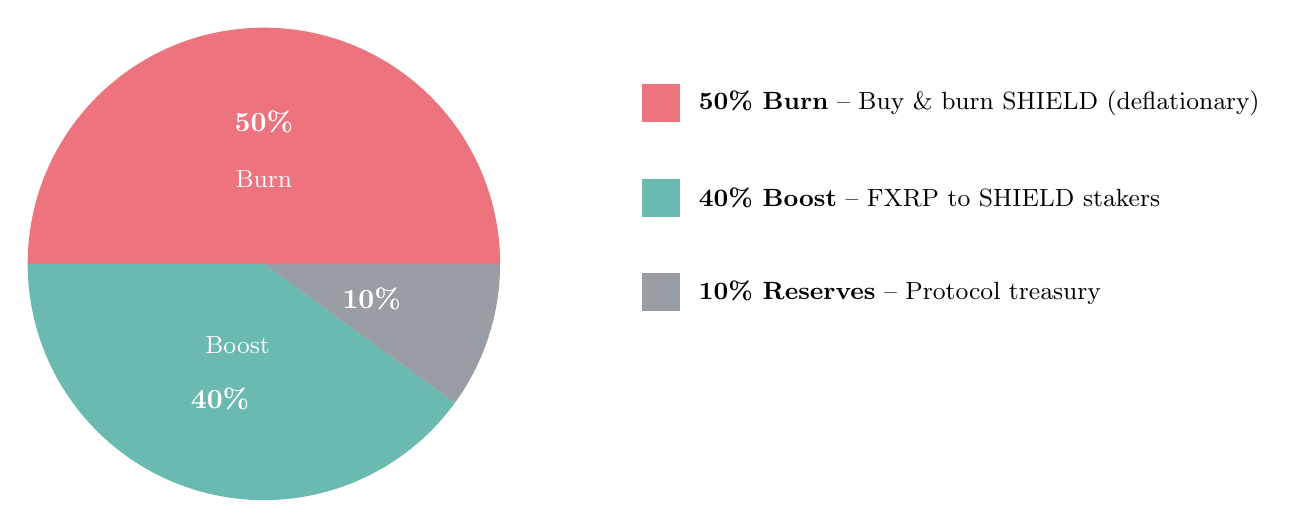
\begin{tikzpicture}[scale=1.2]
    % Pie chart
    \def\radius{2.5}
    
    % 50% Burn (0 to 180 degrees)
    \fill[burnred!70] (0,0) -- (0:\radius) arc (0:180:\radius) -- cycle;
    
    % 40% Boost (180 to 324 degrees)
    \fill[boostgreen!70] (0,0) -- (180:\radius) arc (180:324:\radius) -- cycle;
    
    % 10% Reserves (324 to 360 degrees)
    \fill[reservegray!70] (0,0) -- (324:\radius) arc (324:360:\radius) -- cycle;
    
    % Labels inside pie
    \node[font=\bfseries, white] at (90:1.5) {50\%};
    \node[font=\small, white] at (90:0.9) {Burn};
    
    \node[font=\bfseries, white] at (252:1.5) {40\%};
    \node[font=\small, white] at (252:0.9) {Boost};
    
    \node[font=\bfseries, white] at (342:1.2) {10\%};
    
    % Legend on the right
    \fill[burnred!70] (4,1.5) rectangle (4.4,1.9);
    \node[right, font=\small] at (4.5, 1.7) {\textbf{50\% Burn} -- Buy \& burn SHIELD (deflationary)};
    
    \fill[boostgreen!70] (4,0.5) rectangle (4.4,0.9);
    \node[right, font=\small] at (4.5, 0.7) {\textbf{40\% Boost} -- FXRP to SHIELD stakers};
    
    \fill[reservegray!70] (4,-0.5) rectangle (4.4,-0.1);
    \node[right, font=\small] at (4.5, -0.3) {\textbf{10\% Reserves} -- Protocol treasury};
    
\end{tikzpicture}
\end{center}

\vspace{1em}

\subsection*{SHIELD Token Metrics}

\begin{center}
\renewcommand{\arraystretch}{1.4}
\begin{tabular}{@{} >{\bfseries}l l @{}}
\toprule
\textbf{Property} & \textbf{Value} \\
\midrule
Total Supply & 10,000,000 SHIELD (fixed, can only decrease) \\
Circulating Supply (post-launch) & 8,000,000 SHIELD (80\%) \\
Treasury \& Airdrop Reserve & 2,000,000 SHIELD (20\%) \\
Initial Fair-Launch Price & \$0.01 per \$SHIELD \\
Initial Liquidity & \$150,000 (100\% locked 24 months) \\
Team Allocation & 0\% (no team tokens) \\
VC Allocation & 0\% (no pre-sale) \\
Lock Period & 30 days minimum to receive boost \\
Projected Boost at Scale & +4--7\% additional APY at \$50--100\,M TVL (revenue-dependent, not guaranteed) \\
\bottomrule
\end{tabular}
\end{center}

\vspace{1em}

\begin{tcolorbox}[
    colback=shieldlight,
    colframe=shieldblue,
    boxrule=1pt,
    arc=3pt,
    left=10pt,
    right=10pt,
    top=8pt,
    bottom=8pt,
    title={\textbf{Reserves \& Treasury}}
]
\textbf{Token Reserves:}
\begin{itemize}
    \item 10\% of total SHIELD supply (1,000,000 SHIELD) held in multi-sig treasury
    \item 10\% of all protocol fees routed to reserves
\end{itemize}

\vspace{0.3em}

\textbf{Breakdown of fee reserves:}
\begin{itemize}
    \item \textbf{50\%} $\rightarrow$ Security \& Audits (Hacken, Trail of Bits, bug bounties)
    \item \textbf{30\%} $\rightarrow$ Liquidity Incentives \& Market Making
    \item \textbf{20\%} $\rightarrow$ Community Grants \& Protocol Development
\end{itemize}

\vspace{0.3em}

{\footnotesize Full transparency: \texttt{github.com/shield-xrpfinance/shieldfinance/tree/main/docs}}
\end{tcolorbox}

\vspace{1em}

\begin{tcolorbox}[
    colback=shieldlight,
    colframe=shieldblue,
    boxrule=1pt,
    arc=3pt,
    left=10pt,
    right=10pt,
    top=8pt,
    bottom=8pt
]
\centering
\textbf{The more SHIELD you stake, the more of the 40\% boost pool you receive.}\\[0.3em]
{\small No inflation. No emissions. Pure protocol revenue share.}
\end{tcolorbox}

\newpage

%%%%%%%%%%%%%%%%%%%%%%%%%%%%%%%%%%%%%%%%%%%%%%%%%%%%%%%%%%%%%%%%%%%%%%%%%%%%%%%
% SCALE AND THE LAW OF LARGE NUMBERS
%%%%%%%%%%%%%%%%%%%%%%%%%%%%%%%%%%%%%%%%%%%%%%%%%%%%%%%%%%%%%%%%%%%%%%%%%%%%%%%

\section{Scale and the Law of Large Numbers}
\label{sec:lln}

Shield Finance is a pooled liquid staking protocol. Every FXRP deposited into the vault is automatically delegated across 50--150+ independent Flare validators (current target: top 100 by stake). This pooling directly triggers the \textbf{Law of Large Numbers (LLN)} --- the statistical principle that random performance variations between validators cancel out as the sample size grows.

\begin{center}
\renewcommand{\arraystretch}{1.4}
\begin{tabular}{@{} p{3.2cm} p{4.8cm} p{4.8cm} @{}}
\toprule
\textbf{Benefit} & \textbf{Solo / Small Pool} & \textbf{Shield at Scale (\$50--100\,M TVL)} \\
\midrule
Yield Stability & 3--12\% APY swings (single validator variance) & Within $\pm$0.4\% of network average \\
Effective Slashing Risk & One bad validator can cost 0.1--1\% & Near-zero probability of material loss$^*$ \\
Compounding Efficiency & Gas + rounding losses 0.5--1.5\% yearly & $<$0.01\% loss (amortised across millions) \\
Insurance Fund Size & Negligible in early days & 10\% of fees $\rightarrow$ $>$\$2--3\,M at \$100\,M TVL \\
Liquidity \& Peg & Thin pools $\rightarrow$ slippage/depeg risk & Deep SparkDEX pools $\rightarrow$ $<$0.05\% slippage \\
\bottomrule
\end{tabular}
\end{center}

\vspace{0.3em}

{\footnotesize $^*$ Flare has no delegator slashing --- only validators' self-bonds are penalised (max $\sim$1\%). Pooling reduces any residual risk to a further 100--1000$\times$.}

\vspace{0.5em}

{\footnotesize Scale advantages observed in mature LSTs (Lido, Rocket Pool, Jito, Marinade) and expected for shXRP.}

\subsection*{Historical Tipping Points (Other Chains)}

Historical data from every major liquid staking token shows the same pattern:

\begin{itemize}
    \item $<$10\% of network stake $\rightarrow$ noticeable APY variance
    \item 20--30\% of network stake $\rightarrow$ LLN dominates; yield smoother than native staking
    \item $>$40\% of network stake $\rightarrow$ the LST effectively becomes the chain's ``risk-free rate''
\end{itemize}

Lido (stETH) today holds 29--31\% of all staked ETH and exhibits $<$0.5\% APY deviation from the network average.\textsuperscript{[2]} Solana LSTs (Jito, Marinade) show identical behaviour at 13--14\% of staked SOL.\textsuperscript{[3]}

\subsection*{Built-in Flywheel}

More TVL $\rightarrow$ stronger LLN effects $\rightarrow$ smoother and safer yield $\rightarrow$ attracts more TVL.

This is not marketing --- it is a mathematical consequence of pooled delegation.

\vspace{1em}

{\footnotesize
\textbf{References:}\\
\textsuperscript{[1]} FlareScan delegation leaderboards (Nov 2025)\\
\textsuperscript{[2]} DeFiLlama LST TVL \& APY dashboards (Nov 2025)\\
\textsuperscript{[3]} Blockworks Research --- Solana LST market share (Oct 2025)
}

\newpage

%%%%%%%%%%%%%%%%%%%%%%%%%%%%%%%%%%%%%%%%%%%%%%%%%%%%%%%%%%%%%%%%%%%%%%%%%%%%%%%
% SUMMARY
%%%%%%%%%%%%%%%%%%%%%%%%%%%%%%%%%%%%%%%%%%%%%%%%%%%%%%%%%%%%%%%%%%%%%%%%%%%%%%%

\section{Summary}

\vspace{1em}

\begin{tcolorbox}[
    colback=shieldlight,
    colframe=shieldblue,
    boxrule=2pt,
    arc=5pt,
    left=15pt,
    right=15pt,
    top=12pt,
    bottom=12pt
]

\begin{center}
{\large\bfseries\color{shieldblue} The Shield Finance Value Proposition}
\end{center}

\vspace{0.5em}

Every week the protocol donates FXRP bought with real revenue. 100\% of that donation is distributed pro-rata to SHIELD lockers:

\vspace{0.8em}

\begin{center}
\fbox{%
\parbox{0.85\textwidth}{%
\centering
\vspace{0.5em}
$\displaystyle \text{Boost}_i = B_t \times \frac{L_i}{L}$
\vspace{0.3em}

{\small where $B_t$ = weekly FXRP revenue, $L_i$ = your locked SHIELD, $L$ = total locked SHIELD}
\vspace{0.5em}
}%
}
\end{center}

\vspace{0.8em}

\begin{center}
{\large\bfseries\color{shieldblue} No minting. No inflation. Pure revenue-share.}
\end{center}

\end{tcolorbox}

\vspace{2em}

\subsection*{Key Differentiators}

\begin{multicols}{2}

\textbf{For XRP Holders:}
\begin{itemize}
    \item Instant liquidity (no lock-up)
    \item 5--8\% base APY from real staking
    \item Native XRPL wallet support (Xaman)
    \item 1-click UX (no EVM complexity)
\end{itemize}

\columnbreak

\textbf{For SHIELD Stakers:}
\begin{itemize}
    \item +4--7\% additional APY boost at scale (\$50--100\,M TVL)
    \item Real revenue share (not emissions)
    \item Deflationary tokenomics (50\% burns)
    \item Governance rights (future)
\end{itemize}

\end{multicols}

\vspace{2em}

\subsection*{Security \& Audits}

\begin{center}
\renewcommand{\arraystretch}{1.4}
\begin{tabular}{@{} l l l @{}}
\toprule
\textbf{Audit Firm} & \textbf{Status} & \textbf{Scope} \\
\midrule
Asfalia & Complete (Nov 2025) & Full smart contract audit \\
Hacken & In Progress & Full smart contract audit \\
Trail of Bits & Scheduled Q1 2026 & Comprehensive security review \\
CertiK & Planned post-launch & Full protocol \& economic audit \\
FlareScan & Complete $\checkmark$ & All contracts verified \\
\bottomrule
\end{tabular}
\end{center}

\vspace{2em}

\subsection*{Roadmap}

\begin{center}
\renewcommand{\arraystretch}{1.4}
\begin{tabular}{@{} l l p{7cm} @{}}
\toprule
\textbf{Timeline} & \textbf{Milestone} & \textbf{Description} \\
\midrule
27 Nov 2025 & Testnet Launch (Coston2) & ShXRPVault, StakingBoost, RevenueRouter deployed \\
Dec 2025 & Mainnet Launch & Production deployment on Flare mainnet \\
Q1 2026 & XRPL Smart Accounts & Gasless Flare transactions via XRPL memo encoding \\
Q1 2026 & Multi-Strategy Yield & Kinetic lending + Firelight liquid staking integration \\
Q1 2026 & Trail of Bits Audit & Comprehensive security review \\
Q2 2026 & Governance & On-chain voting for protocol parameters \\
\bottomrule
\end{tabular}
\end{center}

\vspace{1em}

\begin{tcolorbox}[
    colback=shieldlight,
    colframe=shieldblue,
    boxrule=1pt,
    arc=3pt,
    left=10pt,
    right=10pt,
    top=8pt,
    bottom=8pt
]
\textbf{XRPL Smart Accounts (Coming December 2025):} Execute Flare smart contract transactions directly from your XRPL wallet using encoded memo instructions. No EVM wallet required. No gas fees. Powered by Flare Data Connector (FDC) for trustless cross-chain verification.
\end{tcolorbox}

\vspace{2em}

\begin{center}
\rule{12cm}{0.5pt}

\vspace{1em}

{\large\color{shieldblue}\textbf{shyield.finance}}

\vspace{0.5em}

{\color{textgray} Website: shyield.finance \quad | \quad dApp: app.shyield.finance \quad | \quad Twitter: @ShieldFinanceX}

\vspace{2em}

{\Large\color{shieldblue}\textit{Shield Finance --- turning the world's most efficient payment asset\\into the highest-yielding liquid one.}}

\end{center}

\newpage

%%%%%%%%%%%%%%%%%%%%%%%%%%%%%%%%%%%%%%%%%%%%%%%%%%%%%%%%%%%%%%%%%%%%%%%%%%%%%%%
% TECHNICAL APPENDIX
%%%%%%%%%%%%%%%%%%%%%%%%%%%%%%%%%%%%%%%%%%%%%%%%%%%%%%%%%%%%%%%%%%%%%%%%%%%%%%%

\section{Appendix: Smart Contract Architecture}

\subsection*{Contract Overview}

\begin{center}
\renewcommand{\arraystretch}{1.4}
\begin{tabular}{@{} l l p{7cm} @{}}
\toprule
\textbf{Contract} & \textbf{Standard} & \textbf{Purpose} \\
\midrule
ShXRPVault & ERC-4626 & Liquid staking vault with deposit/withdraw \\
ShieldToken & ERC-20 & Governance token with burn function \\
StakingBoost & Custom & Synthetix-style reward accumulator \\
RevenueRouter & Custom & Fee splitting (50/40/10) and swaps \\
VaultController & Access Control & Emergency pause and admin functions \\
\bottomrule
\end{tabular}
\end{center}

\vspace{1.5em}

\subsection*{Deployment Dependency Resolution}

StakingBoost and ShXRPVault have a circular dependency solved via three-step deployment:

\begin{center}
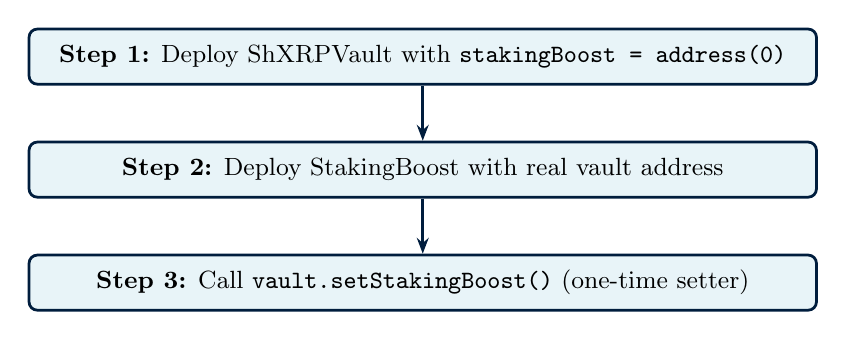
\begin{tikzpicture}[
    node distance=0.7cm,
    box/.style={
        rectangle,
        rounded corners=3pt,
        draw=shieldblue,
        fill=shieldlight,
        line width=1pt,
        minimum height=0.7cm,
        minimum width=10cm,
        text centered,
        font=\small
    },
    myarrow/.style={
        ->,
        >={Stealth[length=2mm]},
        line width=1pt,
        draw=shieldblue
    }
]

\node[box] (step1) {\textbf{Step 1:} Deploy ShXRPVault with \texttt{stakingBoost = address(0)}};
\node[box, below=of step1] (step2) {\textbf{Step 2:} Deploy StakingBoost with real vault address};
\node[box, below=of step2] (step3) {\textbf{Step 3:} Call \texttt{vault.setStakingBoost()} (one-time setter)};

\draw[myarrow] (step1) -- (step2);
\draw[myarrow] (step2) -- (step3);

\end{tikzpicture}
\end{center}

\vspace{1em}

\subsection*{Security Properties}

\begin{itemize}
    \item \textbf{ReentrancyGuard}: All state-changing functions protected
    \item \textbf{Access Control}: Role-based permissions via OpenZeppelin
    \item \textbf{One-Time Setter}: \texttt{setStakingBoost()} cannot be called twice
    \item \textbf{Pausable}: Emergency circuit breaker on vault deposits
    \item \textbf{Non-Custodial}: No admin access to user funds
\end{itemize}

\vspace{0.5em}

{\footnotesize Detailed treasury allocation and boost mechanics maintained in repository (commit-synced with this whitepaper v1.3).}

\vspace{1.5em}

\subsection*{Contract Addresses (Coston2 Testnet --- LIVE)}

\begin{center}
\small
\renewcommand{\arraystretch}{1.3}
\begin{tabular}{@{} l l @{}}
\toprule
\textbf{Contract} & \textbf{Address (Coston2)} \\
\midrule
ShieldToken & \texttt{0x0617A18D1E81f7A34CafDAff3ba2D1f21ccE6616} \\
RevenueRouter & \texttt{0x262Ab80D9e6E09c3D99Bb6bD3d6B093ebDcE0fFB} \\
StakingBoost & \texttt{0xC7C69b4488C9D5c88E14BdC2c14e2C6C2bEE72B4} \\
ShXRPVault & \texttt{0xeBb92e8F1fF38F74Ed2D0fb55d92c2d7C2Cc890e} \\
\bottomrule
\end{tabular}
\end{center}

\vspace{0.5em}

{\footnotesize\textbf{Mainnet addresses:} To be announced December 2025}

\vspace{1em}

\begin{center}
{\footnotesize All contracts verified on FlareScan. View source code at \texttt{github.com/shield-xrpfinance/shieldfinance/tree/main/docs}}
\end{center}

\newpage

%%%%%%%%%%%%%%%%%%%%%%%%%%%%%%%%%%%%%%%%%%%%%%%%%%%%%%%%%%%%%%%%%%%%%%%%%%%%%%%
% INSTITUTIONAL SAFEGUARDS
%%%%%%%%%%%%%%%%%%%%%%%%%%%%%%%%%%%%%%%%%%%%%%%%%%%%%%%%%%%%%%%%%%%%%%%%%%%%%%%

\section*{Institutional Safeguards}

\subsection*{Smart Contract Security}

Shield Finance implements defense-in-depth security architecture:

\begin{itemize}
    \item \textbf{ERC-4626 Standard}: Fully compliant vault implementation ensuring interoperability and auditability
    \item \textbf{OpenZeppelin Contracts}: ReentrancyGuard, SafeERC20, AccessControl, Pausable
    \item \textbf{One-Time Setters}: Critical parameters (StakingBoost address) can only be set once
    \item \textbf{Emergency Controls}: Pausable deposits/withdrawals with multi-sig governance
    \item \textbf{Non-Custodial}: No admin access to user funds; all operations permissionless
\end{itemize}

\vspace{0.5em}

\subsection*{Security Audits}

\begin{center}
\renewcommand{\arraystretch}{1.4}
\begin{tabular}{@{} l l l @{}}
\toprule
\textbf{Auditor} & \textbf{Status} & \textbf{Report} \\
\midrule
Asfalia & Complete (November 2025) & asfalia.io/reports/shield \\
Hacken & In Progress & hacken.io/audits/shield-finance \\
Trail of Bits & Scheduled Q1 2026 & --- \\
Immunefi Bug Bounty & Active & immunefi.com/bounty/shieldfinance \\
\bottomrule
\end{tabular}
\end{center}

\vspace{1em}

\subsection*{Operational Security}

\begin{itemize}
    \item \textbf{Multi-Signature Governance}: 3-of-5 multi-sig for protocol parameter changes
    \item \textbf{Timelock}: 48-hour delay on all governance actions
    \item \textbf{Cold Storage}: Treasury reserves held in hardware wallet multi-sig
    \item \textbf{Annual External Audits}: Commitment to yearly security reviews
\end{itemize}

\newpage

%%%%%%%%%%%%%%%%%%%%%%%%%%%%%%%%%%%%%%%%%%%%%%%%%%%%%%%%%%%%%%%%%%%%%%%%%%%%%%%
% VARA REGULATORY COMPLIANCE
%%%%%%%%%%%%%%%%%%%%%%%%%%%%%%%%%%%%%%%%%%%%%%%%%%%%%%%%%%%%%%%%%%%%%%%%%%%%%%%

\section*{Regulatory Compliance \& Risk Disclosure}

\subsection*{VARA Alignment (Dubai Virtual Assets Regulatory Authority)}

Shield Finance has been designed with consideration for VARA's regulatory framework\textsuperscript{[5]}. The following disclosures are provided for transparency:

\vspace{0.5em}

\textbf{Token Classification.} \$SHIELD is classified as a \textbf{utility token} that provides access to yield-boost functionality within the Shield Finance protocol. It is not designed or intended to represent securities, shares, equity, or ownership in any legal entity.

\vspace{0.5em}

\textbf{Geographic Restrictions.} Front-end access to app.shyield.finance is restricted for UAE IP addresses pending VASP licensing. Users bear sole responsibility for ensuring compliance with local regulations. Smart contract interactions remain permissionless per blockchain design.

\vspace{0.5em}

\textbf{AML/CFT Framework.} While Shield Finance operates as a non-custodial, permissionless protocol, the team maintains:
\begin{itemize}
    \item Transaction monitoring for known sanctioned addresses (OFAC, EU, UN lists)
    \item Cooperation with law enforcement upon valid legal requests
    \item Suspicious Transaction Reporting (STR) capability
    \item MLRO (Money Laundering Reporting Officer) designation for corporate entity
\end{itemize}

\vspace{0.5em}

\textbf{Marketing Compliance.} This whitepaper has been prepared in accordance with VARA Marketing Regulations (effective October 2024)\textsuperscript{[6]}:
\begin{itemize}
    \item All yield projections are based on historical/verifiable on-chain data
    \item No guarantees of returns or profit are made or implied
    \item Risk disclosures are prominently displayed
    \item No FOMO-driven or exaggerated claims
\end{itemize}

\vspace{1em}

\subsection*{Risk Disclosure}

\begin{tcolorbox}[
    colback=burnred!5,
    colframe=burnred,
    boxrule=1pt,
    arc=3pt,
    left=10pt,
    right=10pt,
    top=8pt,
    bottom=8pt
]
\small

\textbf{IMPORTANT: Read carefully before using Shield Finance.}

\vspace{0.5em}

\textbf{Smart Contract Risk.} Despite audits, smart contracts may contain undiscovered vulnerabilities. Loss of funds is possible. Audits reduce but do not eliminate risk.

\vspace{0.3em}

\textbf{Flare Network Risk.} Shield Finance depends on Flare Network infrastructure. Changes to Flare's inflation schedule, FAssets collateralization requirements, or network security could impact yields or fund safety.

\vspace{0.3em}

\textbf{FAssets Bridge Risk.} XRP-to-FXRP bridging via FAssets involves 3--5 day finality periods and depends on collateral providers. Systemic risk exists if collateral becomes insufficient.

\vspace{0.3em}

\textbf{Oracle/Price Feed Risk.} Yield strategies rely on Flare's FTSO (Flare Time Series Oracle) system for price data. Oracle manipulation or downtime could affect protocol operations.

\vspace{0.3em}

\textbf{Liquidity Risk.} Early-stage TVL may result in higher slippage or delayed withdrawals during high-demand periods.

\vspace{0.3em}

\textbf{Regulatory Risk.} DeFi regulation is evolving globally. Future regulatory changes could restrict access or operation of the protocol.

\vspace{0.3em}

\textbf{Economic Risk.} Yield rates depend on Flare network conditions, FAssets rewards, and market dynamics. Projected yields are not guaranteed.

\end{tcolorbox}

\vspace{0.5em}

{\footnotesize This is not an exhaustive list of risks. Users should conduct their own research (DYOR) and consult professional advisors before participating.}

\newpage

%%%%%%%%%%%%%%%%%%%%%%%%%%%%%%%%%%%%%%%%%%%%%%%%%%%%%%%%%%%%%%%%%%%%%%%%%%%%%%%
% REFERENCES
%%%%%%%%%%%%%%%%%%%%%%%%%%%%%%%%%%%%%%%%%%%%%%%%%%%%%%%%%%%%%%%%%%%%%%%%%%%%%%%

\section*{References}

\renewcommand{\arraystretch}{1.5}
\begin{tabular}{@{} l p{12cm} @{}}
{[1]} & Flare Network Staking Rewards --- \texttt{flarescan.com/staking} \\
{[2]} & Kinetic Markets FXRP Lending Pools --- \texttt{kinetic.markets} \\
{[3]} & Firelight Liquid Staking --- \texttt{firelight.fi} \\
{[4]} & Hacken Security Audit (In Progress) --- \texttt{hacken.io/audits/shield-finance} \\
{[5]} & VARA Regulations 2023 + Rulebooks v2.0 (May 2025) --- \texttt{vara.ae/en/regulations} \\
{[6]} & VARA Marketing Regulations (October 2024) --- \texttt{vara.ae/en/marketing-guidelines} \\
{[7]} & Flare FTSOv2 Documentation --- \texttt{docs.flare.network/tech/ftso} \\
{[8]} & FAssets System Documentation --- \texttt{docs.flare.network/tech/fassets} \\
{[9]} & OpenZeppelin Contracts --- \texttt{openzeppelin.com/contracts} \\
{[10]} & ERC-4626 Tokenized Vault Standard --- \texttt{eips.ethereum.org/EIPS/eip-4626} \\
\end{tabular}

\vspace{2em}

%%%%%%%%%%%%%%%%%%%%%%%%%%%%%%%%%%%%%%%%%%%%%%%%%%%%%%%%%%%%%%%%%%%%%%%%%%%%%%%
% DISCLAIMER
%%%%%%%%%%%%%%%%%%%%%%%%%%%%%%%%%%%%%%%%%%%%%%%%%%%%%%%%%%%%%%%%%%%%%%%%%%%%%%%

\section*{Legal Disclaimer}

\begin{tcolorbox}[
    colback=white,
    colframe=textgray,
    boxrule=0.5pt,
    arc=3pt,
    left=15pt,
    right=15pt,
    top=12pt,
    bottom=12pt
]
\small

This whitepaper is for informational purposes only and does not constitute financial, investment, legal, or tax advice. The information provided herein is subject to change without notice.

\textbf{No Investment Advice.} Nothing in this document should be construed as a recommendation to buy, sell, or hold any cryptocurrency, token, or digital asset.

\textbf{Risk Disclosure.} Cryptocurrency investments involve significant risk, including the possible loss of principal. Smart contracts may contain bugs or vulnerabilities. Past performance is not indicative of future results.

\textbf{Regulatory Uncertainty.} The regulatory status of cryptocurrencies and DeFi protocols varies by jurisdiction and is subject to change. Users are responsible for understanding and complying with applicable laws in their jurisdiction.

\textbf{UAE Residents.} This document is not directed at, and the services described herein are not available to, residents of the United Arab Emirates pending VASP licensing. Front-end access is restricted for UAE IP addresses.

\textbf{No Warranties.} Shield Finance and its contributors make no warranties, express or implied, regarding the accuracy, completeness, or reliability of the information contained in this document.

\textbf{Forward-Looking Statements.} This document contains forward-looking statements based on current expectations. Actual results may differ materially from those expressed or implied.

\textbf{Seek Professional Advice.} Users should seek independent legal, financial, and tax advice before participating in any DeFi protocol or acquiring any digital asset.

\vspace{0.5em}

{\footnotesize Whitepaper v1.3 accurate as of November 2025. Repository: \texttt{github.com/shield-xrpfinance/shieldfinance}}

\end{tcolorbox}

\vspace{3em}

\begin{center}
\rule{8cm}{0.5pt}

\vspace{2em}

{\LARGE\color{shieldblue}\bfseries Shield Finance}

\vspace{1em}

{\large\color{textgray}\textit{Turning dormant XRP into sustainable yield\\through transparent, audited infrastructure.}}

\vspace{2em}

{\color{textgray} November 2025 --- Version 1.3 (Testnet Live -- Mainnet December 2025)}

\vspace{1em}

{\scriptsize\color{reservegray} VARA 2025 Standards Aligned (Non-UAE Targeted)}

\end{center}

%%%%%%%%%%%%%%%%%%%%%%%%%%%%%%%%%%%%%%%%%%%%%%%%%%%%%%%%%%%%%%%%%%%%%%%%%%%%%%%
% END DOCUMENT
%%%%%%%%%%%%%%%%%%%%%%%%%%%%%%%%%%%%%%%%%%%%%%%%%%%%%%%%%%%%%%%%%%%%%%%%%%%%%%%

\end{document}
